\documentclass[12pt]{article}

\usepackage{fullpage}
\usepackage{graphicx, rotating, booktabs} 
\usepackage{times} 
\usepackage{natbib} 
\usepackage{indentfirst} 
\usepackage{setspace}
\usepackage{grffile} 
\usepackage{hyperref}
\usepackage{adjustbox}
\setcitestyle{aysep{}}


\singlespace
\title{
\textbf{Testing the Public Goods Theory of Alliances}
	}
\author{Joshua Alley\footnote{Graduate Student,
Department of Political Science, Texas A\&M University.}}
\date{{\normalsize \today}}

\bibliographystyle{apsr}

\begin{document}

\maketitle 

\doublespace



%----------------------------------
\section{Introduction}


\citet{OlsonZeckhauser1966} argue that international alliances are subject to a collective action problem. 
The aggregate capability of an alliance provides security for members. 
But because a treaty cannot exclude members without undermining its purpose, security is a public good. 
Individual members gain security from treaty participation, regardless of their individual contribution. 
Olson and Zeckhauser expect that larger members of the alliance with bear a higher defense burden, because these states value defense from the alliance more. 
Therefore, smaller alliance members free-ride on the contributions of larger partners. 


The prediction that larger alliance members will bear a higher defense burden has been subjected to extensive scrutiny. 
Unfortunately, the standard test regresses military spending as a share of national income on national income. 
This approach places GDP on both sides of the regression, making the models unidentified. 


\citet{PluemperNeumayer2015} attempt to rectify this problem by examining changes in spending among NATO members. 
In their framework, a lack of responsiveness to US and Soviet military spending is evidence of free riding among NATO members.
They find no correlation between the size of a NATO member and free-riding, which they argue contradicts Olson and Zeckhauser. 
However, they do not include the United States in their sample, which omits a crucial data point for testing the size argument.\footnote{Given the focus on responses to US spending, this decision is understandable.}


% So what is the problem here? 
Despite the canonical status of \citet{OlsonZeckhauser1966}, their predictions have not been tested appropriately. 
Regressions with GDP in the outcome and as the key predictor are unidentified. 
\citet{PluemperNeumayer2015} address the identification problem in a way that does not completely test the size prediction. 
There is enough evidence to conclude allied capability allows NATO members spend less on the military \citep{PluemperNeumayer2015, GeorgeSandler2017}.


% by the way, it's mostly NATO
Most tests of free-riding in alliances look at NATO. 
My survey of the literature on alliance participation and military spending found six tests of the public goods theory of alliances outside of NATO. 
All six of those studies include GDP in the independent and dependent variable, creating an identification problem. 


% So it total, there's a lot we don't know
Due to identification problems and the overwhelming focus on NATO, we have limited empirical knowledge of the public goods theory of alliances. 
Understanding of NATO is worthwhile. 
But it is insufficient to assess the overall explanatory power of the public goods theory of alliances. 


% I'm not the first one to address this theory: first comprehensive empirical evidence


% Why we should care
Failures in testing the public goods theory of alliances have two important consequences. 
First, it hinders the accumulation of knowledge. 
Testing predictions from a theory is essential to assessing its explanatory power. 
Without a valid and comprehensive test, the validity of the public goods theory will remain unclear. 


% Why we should care: policy and free riding
If the public goods theory of alliances was only an academic matter, the lack of solid empirical evidence would not be as concerning. 
But the idea of free-riding is ubiquitous in popular and policy debates. 
Charges of free-riding by NATO members are used to question the value of the treaty itself. 
If the public goods theory of alliances has limited explanatory power, charges of free-riding are on shaky ground. 


Establishing the empirical validity of the public goods theory of alliances is necessary for theoretical progress and policy debates. 
Below, I outline two possible solutions to this challenge. 
Both broaden the focus away from NATO, but employ different techniques to examine the role of alliance participant size from 1816 to 2007. 


The approach uses a standard panel data research design, using aggregate measures of alliance participation.
Here, I find no evidence of a conditional relationship between state military spending, changes in allied spending, and state size. 
The second design employs a multilevel model to generate separate estimates for every alliance. 
In the multilevel model, I test Olson and Zeckhauser's prediction that states which contribute more to an alliance should spend more by estimating the impact of increasing alliance contribution on military spending. 
% Summarize aggregate findings here. 


The paper proceeds as follows.
First, I summarize the public goods theory of alliances and its key predictions in more detail.
Then, I describe and summarize the results of panel-data tests of the public goods logic.
The third section describes the multilevel model and associated results. 
The final section assesses aggregate support for the public goods logic, as well as implications for scholars and policymakers. 


\section{The Public Goods Theory of Alliances}


\section{Panel Data Regression}

If Olson and Zeckhauser's argument is correct, smaller states should decrease military spending in response to greater allied military spending. 
This implies a conditional relationship between allied spending, state size, and state military spending. 


\subsection{Absolute Size: GDP}

\begin{figure}
	\centering
		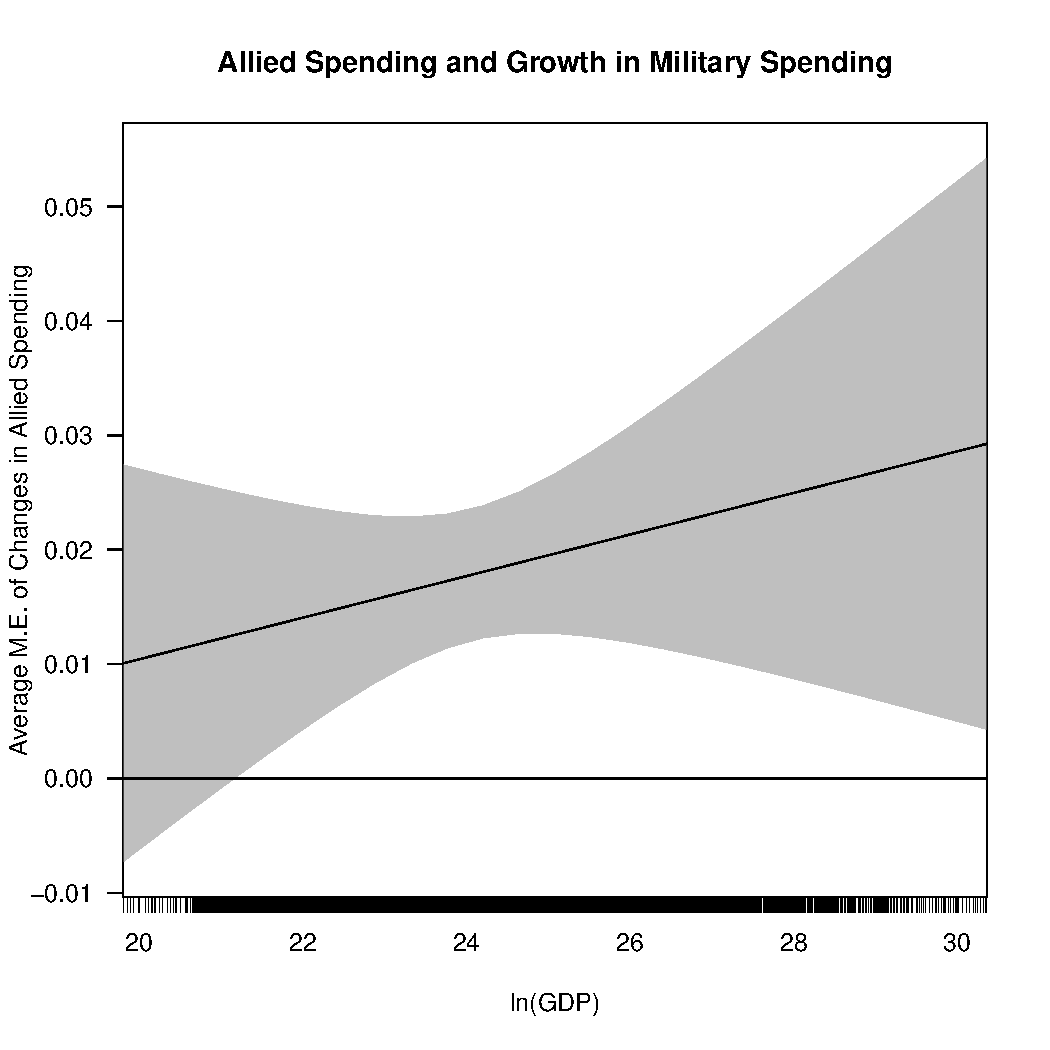
\includegraphics[width=0.95\textwidth]{abs-margins-plot.pdf}
	\label{fig:abs-margins-plot}
	\caption{Average Marginal Effect of increasing allied military spending on a state's military spending, across the range of GDP.}
\end{figure}


\subsection{Relative Size: Alliance Contribution} 


\begin{figure}
	\centering
		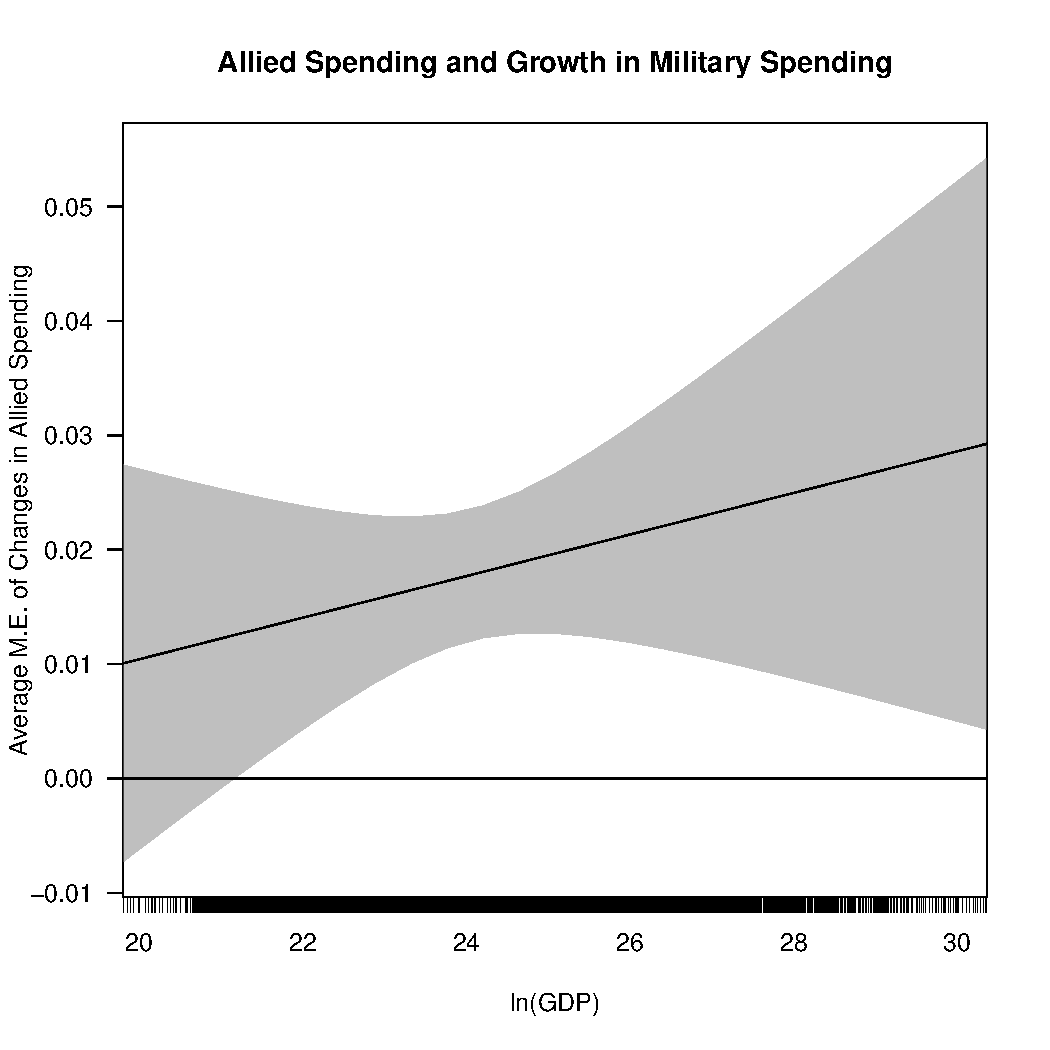
\includegraphics[width=0.95\textwidth]{abs-margins-plot.pdf}
	\label{fig:abs-margins-plot}
	\caption{Average Marginal Effect of increasing allied military spending on a state's military spending, across the average contribution of that state to its alliances.}
\end{figure}


\section{Multilevel Model}


\section{Conclusion}


\singlespace


%\bibliography{C:/Users/jkalley14/Dropbox/Research/MasterBibliography}  
\bibliography{C:/Users/Josh/Dropbox/Research/MasterBibliography} 





\end{document}


